\documentclass[authoryear,preprint,review,12pt]{elsarticle}


\usepackage[a4paper, total={6in, 8in}]{geometry}


\usepackage{amsmath,amssymb}
% Natbib package is auto-loaded by elsarticle.cls
\usepackage{color}
% Hyperref for hyperlinked cross references
\usepackage{hyperref}
% Remark and argmin
\newtheorem{remark}{Remark}
\DeclareMathOperator*{\argmin}{argmin}

\journal{Computers and Chemical Engineering}

\begin{document}
\scrollmode

% *** FRONT MATTER: TITLE, AUTHORS, ABSTRACT ***
% **********************************************
\begin{frontmatter}

% TITLE
\title{Simultaneous Sensor and Actuator Placement for Contaminant Detection and Mitigation in Water Distribution Networks}
%\title{Control of Hyperbolic PDE systems using Reduced Order
%Models and Approximate Dynamic Programming}
% AUTHORS
\author[iitm]{Suhas Gundimeda}
\author[iitm]{Venkata Reddy Palleti}
\author[iitm]{Shankar Narasimhan}

% ADDRESSES
\address[iitm]{Department of Chemical Engineering, Indian Institute of Technology Madras, Chennai 600036, India}
%\fntext[abb]{Currently at: ABB Corporate Research Center, Bhoruka Tech Park, Whitefield Main Road, Bangalore 560048, India}
%\cortext[cor1]{Corresponding author; Email: sridharkrn@iitm.ac.in; Phone: [+91] (44) 22574177}

% ABSTRACT
\begin{abstract}
Water Distribution Networks (WDNs) are considered to be part of the critical infrastructure of any city. WDNs are often exposed to either  accidental or intentional  contamination. Therefore,
it is very important to protect the public form such kinds of incidents. These contaminants can be detected by deploying sensors in the work. Once the sensors detects the presence of a contamination, it is also necessary to take appropriate actions in order to mitigate the effects of contaminations. Therefore, in this paper, we propose an optimal simultaneous sensor and actuator  placement for contamination detection and mitigation in WDNs. A multi-objective mixed integer linear
 optimization formulation is proposed to obtain the optimal sensor and actuator placement. The proposed method is demonstrated on the real urban water distribution system.

\end{abstract}

% KEYWORDS
\begin{keyword}
Water distribution networks, observable sensor network, actuator network, contamination detection and mitigation.
\end{keyword}

\end{frontmatter}

% *** MAIN CONTENT OF THE PAPER STARTS HERE ***
% *********************************************
\section{Introduction}

% These networks are identified
% to be vulnerable to contamination \cite{Kessler1998,}.


Water Distribution Networks (WDNs) are networks of pipes, tanks, pumps,
valves, and other components that are used to distribute water from
sources, like reservoirs, to consumers. The  topology of the network, number of consumer nodes, loading conditions, hydraulic elements etc make the control of a water distribution system a
difficult task and makes it highly vulnerable to contamination \citep{Kessler}.  WDNs are often susceptible to either accidental or  intentional contamination. Accidental contamination occurs due to  system deficiencies (e.g, cross connections, pipeline breakage) and intentional contamination occurs as a result of deliberate acts of chemical or biological intrusions. Introduction of  chemical or biological agents in WDN can damage public health. After  9/11 attacks in United States, the
concern over  possible terrorist attacks on WDN has increased and can be considered as the most serious threat to WDNs \citep{BWSN}. Hence, it is very important to detect such kinds of attacks as quickly as possible  and it is also necessary to take appropriate actions to mitigate the effects of a contamination event. Suggested detection and response methods are varied, and one such is the placing of online sensors and actuators (or shut-off valves) for detection and containment of   contaminants.
The sensors can be used to detect the contaminants, and the actuators are useful to shut down the network to  prevent further spread of contaminants. Therefore, in this paper we propose a methodology to obtain an  optimal sensor and actuator placement  for contaminant detection and mitigation of the contamination effects.


The problems of contaminant detection in WDNs and appropriate response to a contamination event have been addressed in literature. Numerous procedures are available in the literature for the
 contamination detection problem. However, very few studies are available with respect to the problem of response to  contamination events. Several optimization algorithms have been proposed for the problem of sensor placement for contamination detection in WDNs. Single objective optimization problems\citep{Kessler, LEE, BERRY_FLEISCHER,  kumar} are solved by considering  objectives for maximizing the demand coverage,  maximizing the likelihood detection and minimizing the elapsed
  time between the injection and detection of contaminants. Further, multi-objective optimization problems \citep{BWSN, rico2007water,  Preis2008-Multiobjective, Watson04} have been solved by considering  objectives for minimizing the time of detection, minimizing the contaminated volume consumed prior to detection, population at risk etc. The problem of contamination source identification based on deployed sensor measurements have been reported \citep{mann2012real,Laird}. Sensor placement
  algorithm using the principle that there must exist a unique non-zero set
of sensors for each of the vulnerable nodes was developed by \cite{Palleti2016246}. In this paper,  the graph abstraction of water distribution networks with vulnerable nodes representing
multiple real nodes and used sets of affected nodes to find a viable sensor placement.

%Recently, the problem of sensor placement, which ensures observability and identifiability conditions has also been studied by . % TODO

Although, design of a sensor network to detect and identify intentional contamination of a WDN is important, it is also necessary to consider the potential action that one can take to mitigate
the effect of the contaminant. Once the sensor network detects the presence of  a contaminant, U.S. Environmental Protection Agency's (USEPA) response protocol toolbox \citep{USEPA2004a} provides recommendations for implementation of specific responses to minimize the effect of contamination event. This protocol includes the detection, source identification followed by consequence management strategies. Various researchers have developed  methodologies related to the detection and source
 identification problems as described earlier. Once a contaminant has been detected, water utilities must evaluate the response to the contamination so that potential impact to the public can be minimized.  These consequence management strategies may include: (1) public notification, (2) isolation and containment of a contaminant through valve operations \citep{USEPA2004a}, (3) flushing the contamination system, and (4) combinations of isolation, notification, and flushing \citep{USEPA2004b}.
 Very few studies are available  with respect to the  mitigating actions that would be taken after detecting the presence of contaminant in the WDN \citep{Poulin2008-heuristic, Poulin-2010, Preis2008-Multiobjective,  Guidorzi2009-Amultiobjective, Alfonso2010-MultiobjectiveOptimization} . Heuristic  procedures are proposed   for isolating a contaminated area through the simultaneous closure of a number of valves in the system, assuming an unlimited number of response teams and subsequent
 removal of the contaminant by unidirectional
flushing \cite{Poulin2008-heuristic, Poulin-2010} . \cite{Preis2008-Multiobjective} proposed a multi-objective approach with the aim of minimizing the number of operations to be performed and
to reduce the consumption of contaminated water by consumers for a given  specific contamination event. Such an approach is  useful only when complete knowledge of the contaminant history is known (in terms of intrusion location,  duration and quantity of contaminant injected). Similarly,   multi-objective procedures were proposed  to identify the minimum number of operations that minimize the contaminated water consumption \citep{Guidorzi2009-Amultiobjective, Alfonso2010-MultiobjectiveOptimization}.  These approaches \citep{Guidorzi2009-Amultiobjective, Alfonso2010-MultiobjectiveOptimization}  have not considered the characteristics of the contamination event (i.e, location, duration and quantity of contaminant introduced). Later,  the problem of optimal scheduling of device activation in order to minimize the consumption of contaminated water after the detection of a contaminant has been studied by \cite{Alvisi345-Nearoptimal}.

The previous studies focused on operational strategies to be implemented in the event
of a contaminant detection assuming that valves are already present in the network.
The design problem of optimal valve placement to minimize  the
effects of  contamination events has not been reported in the literature.
But recently, \cite{palleti_actuator_2018} proposed a methodology for design of actuator network
for a given sensor network to mitigate contamination effects in
WDNs. In their work, shut-off valves
are placed on optimal number of pipes so that it
is possible to shutdown the network to prevent the uncontaminated
part of the network from the contaminated network.  Further, they design the actuator
network assuming that the sensor network design has already been carried out and locations of
sensors are known a priori. It means that the sensor and actuator network designs
are carried out independently and they are decoupled.  In contrast to this work,
in this paper, we obtain a sensor and actuator placement simultaneously for detection and
mitigation of contamination effects.  Therefore, in this work we propose a multi-
objective mixed integer linear optimization formulation is proposed to determine the simultaneous
optimal sensor and actuator network. Also, we hypothesize that simultaneous sensor
and actuator planning can be achieved and is more efficient than
iterative non-linear optimization sequentially solving the two placement problems,
%Check the appropriateness of the following. TODO
i.e. these are not independent problems, and these can be formulated as an integer
linear program and solved.


%\subsection{Previous work}
%.
%
%Given the sensor network, a linear optimization model for placement of minimal number
%of actuators on edges to
%achieve shut-down of network to contain contaminant was performed in [2]. The current work combines these methods in a multi-objective optimization formulation.
%
%An approach in [4] attempts to optimize different objectives: maximizing detection likelihood and minimizing expected time to detection and solves it using genetic algorithms.
 The current work assumes both of these objectives are binary, i.e. no time delay in detection and accurate sensing.
%
%%TODO Do a review of the review papers cited
%
%
%We first develop a formulation and algorithm for each case, implement a simulation in MATLAB, and compare with test case results from previous works to check veracity and improvement.
%\section{Problem Description}



\section{Problem Description}

% TODO, commented out is the old problem Description
%Specifications of the water distribution network
% are provided as vulnerable nodes, demand nodes, and the sparse adjacency matrix.
% The demand nodes are the nodes we want to prevent the contamination of.
% Time-delay in sensors of contaminant sensing, lengths of pipes, accuracy of sensing,
% identification of which vulnerable node was affected, etc.
% can be added onto this work easily, and are not considered here.
The water distribution network is represented as a deterministic weighted directed graph,
$G(V,E)$, where $E$ represents the edges or connections, and $V$ represents the vertices or
nodes.
Nodes are used to represent sources, such as reservoirs or tanks from where water is supplied,
as well as demand points where water is consumed and taken out of the network.
All the junctions of pipes, such as those from pipes dividing or combining are also regarded as nodes.
Pipes, valves, pumps, and other connections are represented as edges in the graph.
A typical city's WDN has several hundred nodes and edges.
Intentional contamination generally only occurs at sources - tanks, reservoirs, fire hydrants.
Unintentional contamination can typically occur at any point in the WDN.
In this work, we develop techniques that can be used for the general case, where any set of nodes in the network can be contaminated.
These potential sites of intrusion are referred to as vulnerable nodes.
%The following simplifying assumptions are made in designing a sensor and actuator placement strategy for mitigation of contamination:

\subsection{Assumptions}
\begin{itemize}
    \item We are given complete information about the network - (sparse) adjacency matrix,
        set of nodes vulnerable to contamination,
        set of nodes which should be prevented from contamination (demand nodes).
    \item Each affected node and sensor satisfies all conditions for sensors to identify
        the presence of contaminant, such as concentration of contaminants, flow rate, sensitivity of sensor, etc.\\
    \item This identification of contaminant is instant, binary and without error - neither false positives or false negatives.
    \item There is no time delay in communication, processing and actuation to stop spread.
\end{itemize}
All of the vulnerable nodes are infected (not necessarily at the same time) - case 1.
A subset of vulnerable nodes are contaminated - this required a modified solution - case 2.

\subsection{Requirements of a solution} % TODO
A distribution of sensors on nodes and actuators on edges such
that an attack on a subset of vulnerable nodes can be identified and
the network shut down.

Three \hyperref[sec:Scenarios]{scenarios} with different and progressive requirements
of a solution are explored in this work, with the differences in formalism illustrated
with an example network.


%Secondary requirement %(same as in \cite{palleti_actuator_2018}): % TODO verify that we should not cite
%A sensor and actuator placement strategy that might allow for initial
%contamination of some demand nodes, but will stop any further contamination
%to all demand nodes.




%\subsection{Case study network}
% TODO
%\textcolor{red}{This has to move to the end: No case study in the procedure}
%
%The algorithms were tested on a benchmark abstraction of an urban WDN; of Bangalore city, India.
%\begin{figure}[ht]
%    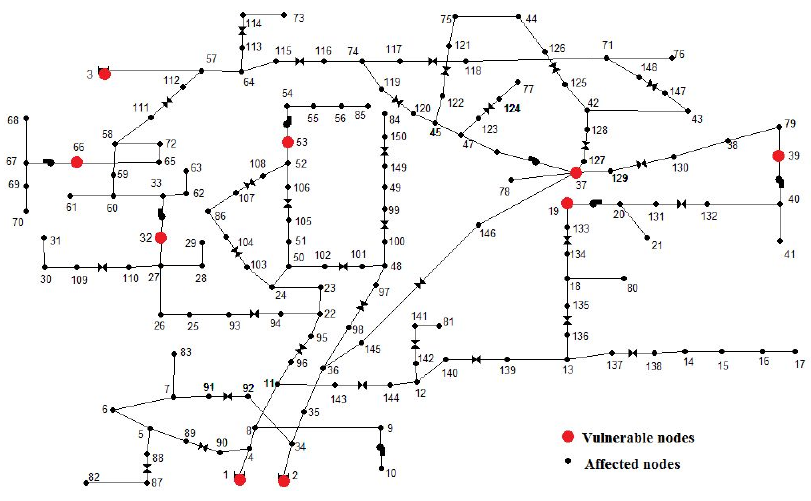
\includegraphics[width=\linewidth]{images/bangalore_vuln_venkat}\caption{Layout of bangalore network, where nodes 1, 2, 3 are reservoirs and
%the six others shown are pumps}
%\end{figure}
% It has 3 reservoirs and 6 pumps, which are considered vulnerable
%nodes. 24 demand nodes are presented in the network. The network consists
%of 116 pipes, 29 control valves, 3 on-off valves and 7 pumps. The
%primary purpose of the network is to supply the water to all demand
%nodes.
%
%
%
%The network is assumed to be static, and the hydraulic results at
%00:00 hours after EPANET simulation are considered for this work.
%All of the results are produced using no more hydraulic information
%then directed connectivity results. All pipes are assumed to be of
%length 1.


\section{Scenarios \label{sec:Scenarios}}


\subsection{Scenario of vacuum pipes \label{sub:Scenario-1:vacuum}}
\subsubsection{Key assumptions} % TODO maybe 'scenario description' is better?
\begin{itemize}
    \item Shutting down the network effectively stops the contaminant
beyond the actuator as well.
    \item Finite amount of contaminant is allowed reach the demand nodes} % TODO Look into separate scenario for this
\end{itemize}

In this simpler scenario, there are no additional constraints on the actuator
placement problem beyond that of actuator edges being a min-cut of
the entire graph. That is, the removal of the pipes in the water distribution
network corresponding to the set of actuator edges must partition the
network into two - one with all the vulnerable nodes, and one with all the demand nodes.
We assert that the sensor and actuator placement problems are independent. % TODO Proof?
As long as the sensor network detects the contaminant before it
reaches the demand nodes and the actuation happens immediately, no demand node is compromised.
But without additional constraints, this is not guaranteed viz. the
formulation presented here minimizes the number of sensor nodes even at the
cost of late (post-compromise) detection.

\subsubsection{Formulating the problem as  Mixed Integer Linear Program (MILP)}
\textcolor{red}{Suhas:what is the base problem . I am guessing that the following is the base problem for all the cases. Venkat, yes, but this is just the simplest scenario.} % TODO
A binary integer optimization problem is presented:

\begin{eqnarray}
\begin{aligned}
\text{PROBLEM I:}~~ min & (\sum x_{i}+\sum z_{i})\\
\text{s.t.}~& \mathbf{A}
p
 \leq \mathbf{b}\\
& \mathbf{A_{eq}}p =  \mathbf{b_{eq}}
\end{aligned}
\end{eqnarray}

%\begin{eqnarray}
%\begin{aligned} \text{PROBLEM II:}~~~ & \underset{x, y}{\text{min}}& & \sum_{k=1}^{m}y_{k} \\
%& \text{s.t.} & &(J^Tx)_k \leq y_k\\
%& & &-(J^Tx)_k \leq y_k\\
%& & & x_i = 0, ~~\forall i \in S \\
%& & &  x_j = 1, ~~ \forall j \in D  \\
%& & &  x_i\in\{0,1\}, \ y_k \in\{0,1\} \\
%\label{formulation}
%\end{aligned}
%\end{eqnarray}


Where, $  p=\begin{bmatrix}
 \mathbf{x} & \mathbf{y} & \mathbf{z} \end{bmatrix}^{T}$

$\mathbf{x}\equiv[x_{i}]$ is 1 if there exists a sensor at
$i^{th}$node, 0 otherwise.

$\mathbf{y}\equiv[y_{i}]$ is 1 if $i^{th}$node is in the demands
side of the actuators, 0 otherwise.

$\mathbf{z}\equiv[z_{i}]$ is 1 if there exists an actuator at $i^{th}$edge,
0 otherwise.

Hence the vector $\left[\mathbf{\begin{array}{ccc}
\mathbf{x} & \mathbf{y} & \mathbf{z}\end{array}}\right]$ is of length $2*N+E$. % TODO define N and E

$A=\left[\begin{array}{cc}
A_{1} & \mathbf{0}\\
\mathbf{0} & A_{2}
\end{array}\right]$, $A=\left[\begin{array}{cc}
A_{eq1} & \mathbf{0}\\
\mathbf{0} & A_{eq2}
\end{array}\right]$, $b=\left[\begin{array}{c}
b_{1}\\
b_{2}
\end{array}\right]$, $b_{eq}=\left[\begin{array}{c}
b_{eq1}\\
b_{eq2}
\end{array}\right]$.

$A_{1}$ is a matrix of vulnerable nodes versus affected nodes, with
$A_{1ij}=-1$ if $i^{th}$ vulnerable node affects the $j^{th}$ node
in graph.

$A_{2}=\left[\begin{array}{cc}

J & I_{E\times E}\end{array}\right]$ where $J$ is the incidence matrix.


$b_{1}=\left[\begin{array}{c}
.\\
.\\
.\\
-1\\
.\\
.\\
.
\end{array}\right]$,
$b_{2}=\left[\mathbf{O}\right]$. This links the partitioning variables
$\mathbf{y}$ to the variables in the cost function, $\mathbf{z}$.


$A_{eq1}=b_{eq1}=\mathbf{O}$


$A_{eq2}$, $b_{eq2}$ provide bounds to force the decision variables
to reality, i.e. the demand nodes being in the second partition and
the vulnerable nodes being in the first.


\subsubsection{Small network example}

Consider the graph represented by \ref{fig:small_network}, with demand node 6 and
vulnerable nodes 1 and 2.

\begin{figure}[ht]
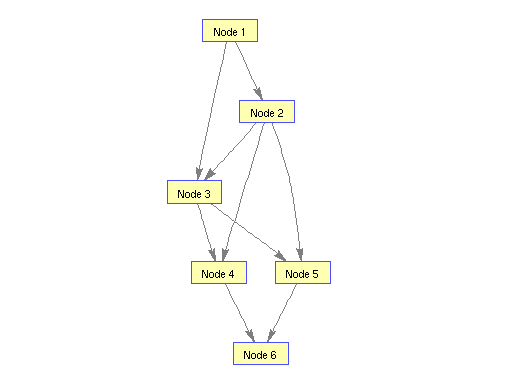
\includegraphics[scale=0.75]{images/testGraph}\caption{The example graph with 6 nodes and 9 edges}
    \label{fig:small_network}
\end{figure} % TODO change to venkat's example network


Formulating as binary integer optimization problem:

\begin{eqnarray*}
min & (\sum x_{i}+\sum z_{i})\\
sub\\
\mathbf{A}\left[\begin{array}{c}
\mathbf{x}\\
\mathbf{y}\\
\mathbf{z}
\end{array}\right] & \leq & \mathbf{b}\\
\mathbf{A_{eq}}\left[\begin{array}{c}
\mathbf{x}\\
\mathbf{y}\\
\mathbf{z}
\end{array}\right] & = & \mathbf{b_{eq}}
\end{eqnarray*}


Hence the vector $\left[\mathbf{\begin{array}{ccc}
\mathbf{x} & y & z\end{array}}\right]$ is of length $2*N+E=21$.

$A=\left[\begin{array}{cc}
A_{1} & \mathbf{0}\\
\mathbf{0} & A_{2}
\end{array}\right]$, $A=\left[\begin{array}{cc}
A_{eq1} & \mathbf{0}\\
\mathbf{0} & A_{eq2}
\end{array}\right]$, $b=\left[\begin{array}{c}
b_{1}\\
b_{2}
\end{array}\right]$, $b_{eq}=\left[\begin{array}{c}
b_{eq1}\\
b_{eq2}
\end{array}\right]$.\\

$A_{1}$ is a matrix of vulnerable nodes versus affected nodes, with $A_{1ij}=-1$ if $i^{th}$ vulnerable node affects the $j^{th}$ node in graph.\\ % TODO ask about using 'vs.' and 'versus'


\scalebox{0.8}{
$A_{1}=\left[\begin{array}{ccccccccccccccccccccc}
-1 & -1 & -1 & -1 & -1 & -1 & 0 & 0 & 0 & 0 & 0 & 0 & 0 & 0 & 0 & 0 & 0 & 0 & 0 & 0 & 0\\
0 & -1 & -1 & -1 & -1 & -1 & 0 & 0 & 0 & 0 & 0 & 0 & 0 & 0 & 0 & 0 & 0 & 0 & 0 & 0 & 0
\end{array}\right]$
}\\


$b_{1}=\left[\begin{array}{c}
-1\\
-1
\end{array}\right]$\\



$A_{eq1}=b_{eq1}=\mathbf{O}$\\

The following maps the actuator placement problem to one of classification
into source or demand partition.


	\scalebox{0.8}{

$A_{2}=\left[\begin{array}{cc}
J & I_{E\times E}\end{array}\right]=\left[\begin{array}{ccccccccccccccc}
-1 & 1 & 0 & 0 & 0 & 0 & -1 & 0 & 0 & 0 & 0 & 0 & 0 & 0 & 0\\
-1 & 0 & 1 & 0 & 0 & 0 & 0 & -1 & 0 & 0 & 0 & 0 & 0 & 0 & 0\\
0 & -1 & 1 & 0 & 0 & 0 & 0 & 0 & -1 & 0 & 0 & 0 & 0 & 0 & 0\\
0 & -1 & 0 & 1 & 0 & 0 & 0 & 0 & 0 & -1 & 0 & 0 & 0 & 0 & 0\\
0 & -1 & 0 & 0 & 1 & 0 & 0 & 0 & 0 & 0 & -1 & 0 & 0 & 0 & 0\\
0 & 0 & -1 & 1 & 0 & 0 & 0 & 0 & 0 & 0 & 0 & -1 & 0 & 0 & 0\\
0 & 0 & -1 & 0 & 1 & 0 & 0 & 0 & 0 & 0 & 0 & 0 & -1 & 0 & 0\\
0 & 0 & 0 & -1 & 0 & 1 & 0 & 0 & 0 & 0 & 0 & 0 & 0 & -1 & 0\\
0 & 0 & 0 & 0 & -1 & 1 & 0 & 0 & 0 & 0 & 0 & 0 & 0 & 0 & -1
\end{array}\right]$ }\\

 where $J$ is the incidence matrix.

$b_{2}=\left[\mathbf{O}\right]$. This links the partitioning variables
$\mathbf{y}$ to the variables in the cost function, $\mathbf{z}$.
An edge between two different partitions causes the cost function
to assume the presence of an edge.

$A_{eq2}$, $b_{eq2}$ provide bounds to force the decision variables
to reality, i.e. the demand nodes being in the second partition and the vulnerable nodes being in the first. \\

$A_{eq2}=\left[\begin{array}{ccccccccccccccc}
1 & 0 & 0 & 0 & 0 & 0 & 0 & 0 & 0 & 0 & 0 & 0 & 0 & 0 & 0\\
0 & 1 & 0 & 0 & 0 & 0 & 0 & 0 & 0 & 0 & 0 & 0 & 0 & 0 & 0\\
0 & 0 & 0 & 0 & 0 & 1 & 0 & 0 & 0 & 0 & 0 & 0 & 0 & 0 & 0
\end{array}\right]$; $b_{eq2}=\left[\begin{array}{c}
0\\
0\\
1
\end{array}\right]$\\


\subsubsection{Results and verification}

\begin{figure}[ht]
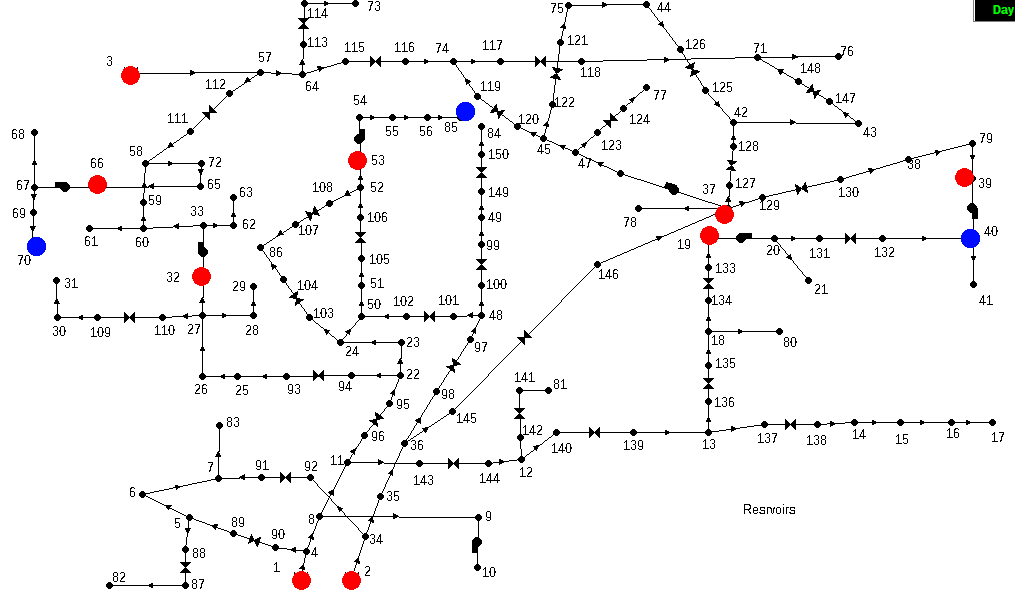
\includegraphics[scale=0.4]{images/netowrkSensorsOnly}\caption{Graph abstraction with vulnerable nodes in red and sensors in blue.}
\end{figure}


\begin{table}[ht]
\centering{}%
\begin{tabular}{|c|c|}
\hline
Vulnerable Nodes & Sensor Nodes\tabularnewline
\hline
\hline
1 & 41, 70, 85\tabularnewline
\hline
2 & 41, 85\tabularnewline
\hline
3 & 70\tabularnewline
\hline
19 & 41\tabularnewline
\hline
32 & 70\tabularnewline
\hline
37 & 41\tabularnewline
\hline
39 & 41\tabularnewline
\hline
53 & 85\tabularnewline
\hline
66 & 70\tabularnewline
\hline
\end{tabular}\caption{Vulnerable nodes and their corresponding sensor nodes}
\end{table}


It takes three sensors to detect contaminant with no other requirements.

This is the same as \cite{Palleti2016246}.

The closing of network requires 12 actuators: on edges 1, 4, 30, 37,
39, 47, 49, 50, 64, 81, 149, 154.

\begin{figure}[ht]
\begin{centering}
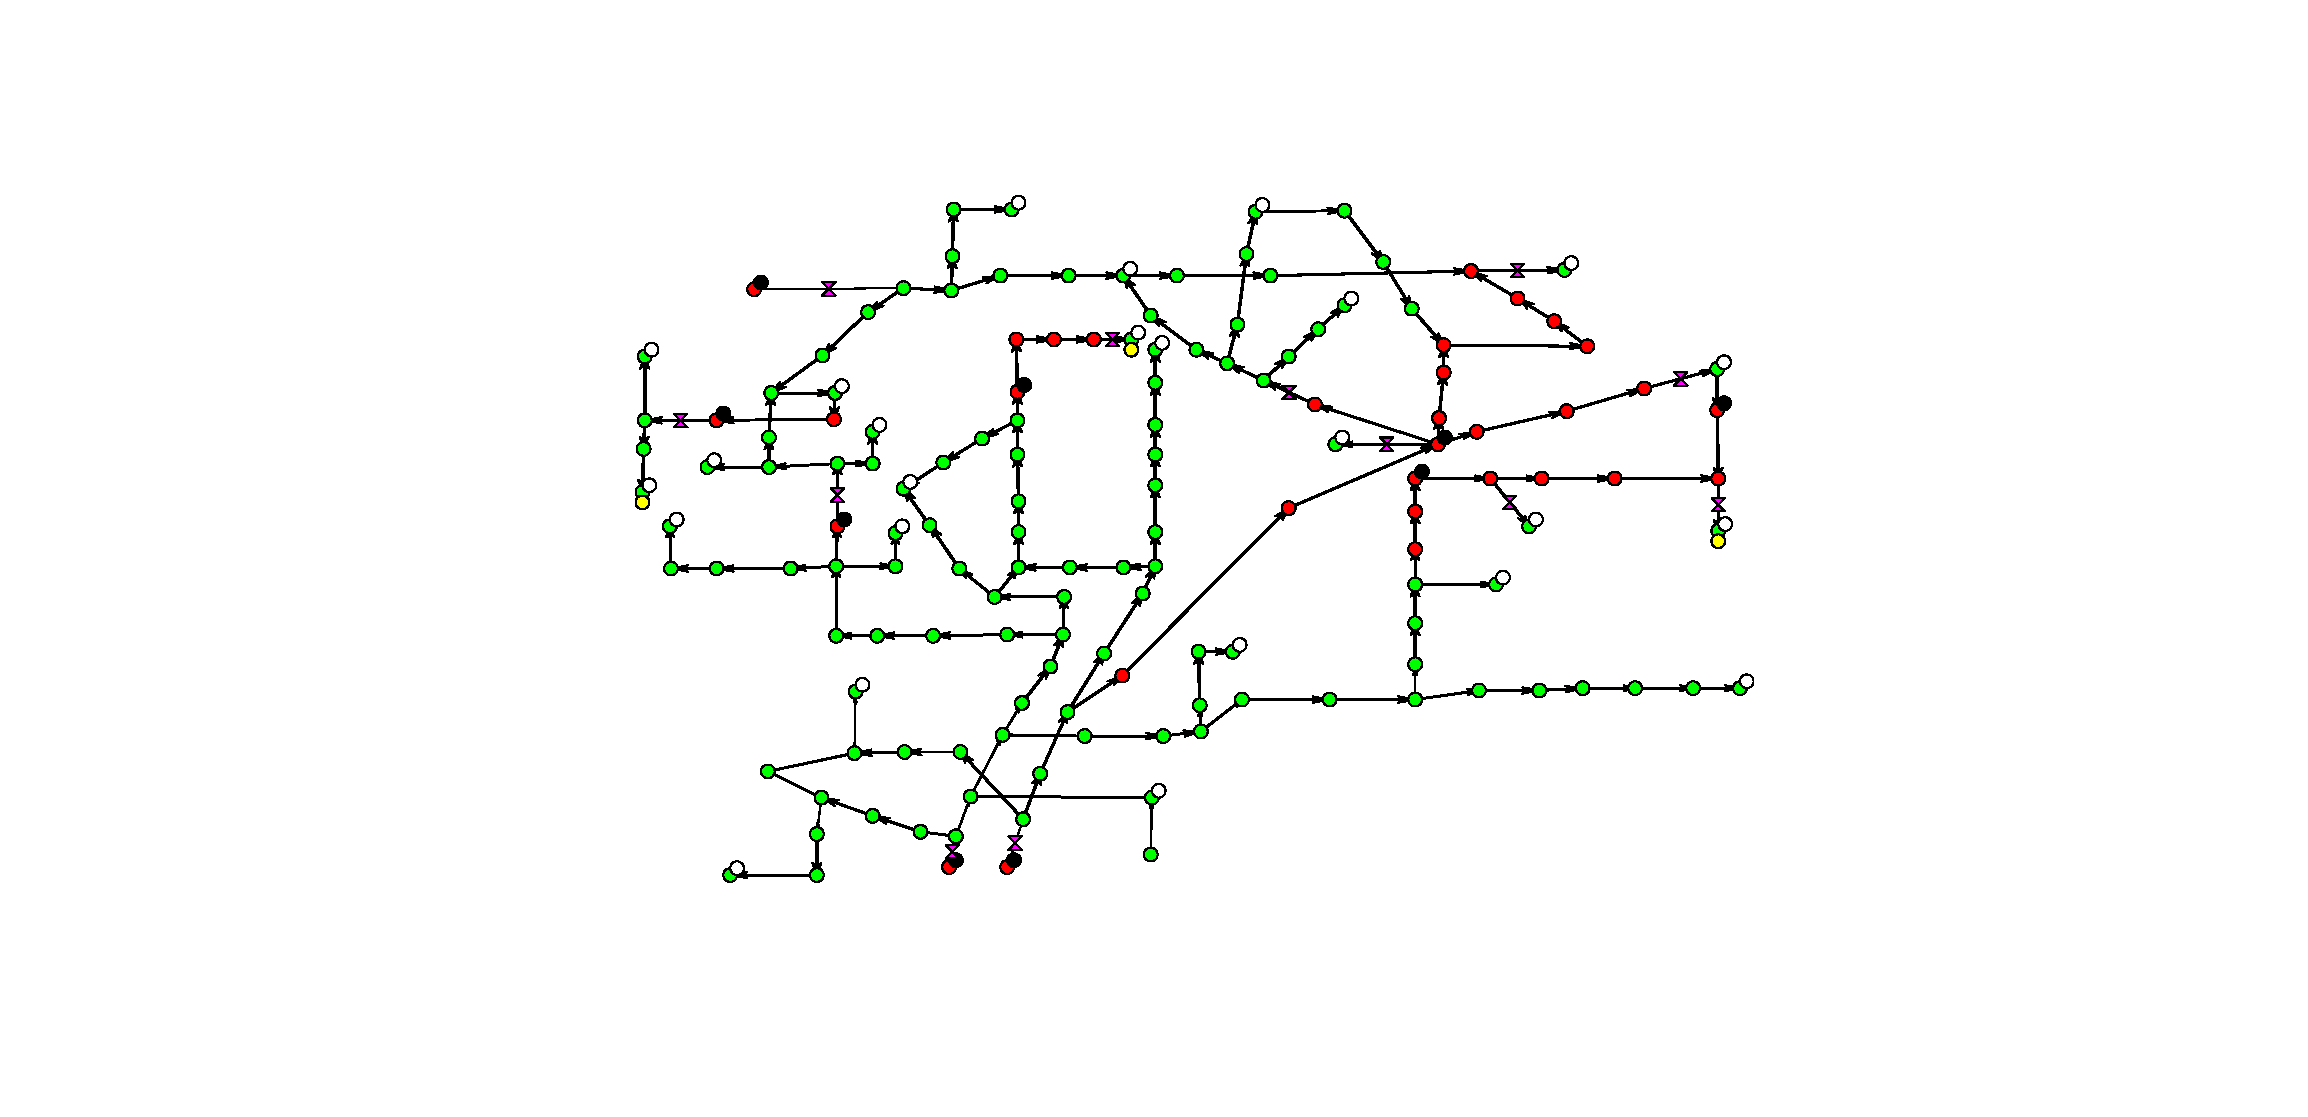
\includegraphics[width=\linewidth]{images/multiobj_indep}\caption{Results of independent placement case}

\par\end{centering}

\end{figure}







\subsection{Scenario of simultaneous attack \label{sub:Scenario-2:containment}}
\subsubsection{Key assumptions}
\begin{itemize}
    \item  The contaminant must be contained in the vulnerable side
    of actuator network.
    \item Contamination attacks occur on all vulnerable nodes at once.
\end{itemize}
This case is not trivial as the positions of the sensors must be used
as input, i.e. time-dependent total spread of each contaminant must be on the contained at time of actuation.


\subsubsection{Formulation}

Formulating as binary integer optimization problem:

\begin{eqnarray*}
min & (\sum x_{i}+\sum z_{i})\\
sub\\
\mathbf{A}\left[\begin{array}{c}
\mathbf{x}\\
\mathbf{y}\\
\mathbf{z}\\
a\\
\mathbf{w}
\end{array}\right] & \leq & \mathbf{b}\\
\mathbf{A_{eq}}\left[\begin{array}{c}
\mathbf{x}\\
\mathbf{y}\\
\mathbf{z}\\
a\\
\mathbf{w}
\end{array}\right] & = & \mathbf{b_{eq}}
\end{eqnarray*}


Where $\mathbf{x}\equiv[x_{i}]$ is 1 if there exists a sensor at
$i^{th}$node, 0 otherwise.

$\mathbf{y}\equiv[y_{i}]$ is 1 if $i^{th}$node is in the demands
side of the actuators, 0 otherwise.

$\mathbf{z}\equiv[z_{i}]$ is 1 if there exists an actuator at $i^{th}$edge,
0 otherwise.

$a$ is a decision variable which stores the maximum distance the
set of sensors are to the set of vulnerable nodes.

$\mathbf{w}\equiv[w_{i}]$ is 1 if $i^{th}$node is in the demands
side of the actuators, a large number($N$) otherwise.

$M$ is a large number.

Hence the vector $\left[\mathbf{\begin{array}{ccccc}
\mathbf{x} & y & z & a & w\end{array}}\right]$ is of length $3*N+E+1$.

$A=\left[\begin{array}{ccc}
A_{1} & \mathbf{0} & \mathbf{0}\\
\mathbf{0} & A_{2} & \mathbf{0}\\
\mathbf{} & A_{3}
\end{array}\right]$, $A=\left[\begin{array}{ccc}
A_{eq1} & \mathbf{0} & \mathbf{0}\\
\mathbf{0} & A_{eq2} & \mathbf{0}\\
\mathbf{0} & A_{eq3}
\end{array}\right]$, $b=\left[\begin{array}{c}
b_{1}\\
b_{2}\\
b_{3}
\end{array}\right]$, $b_{eq}=\left[\begin{array}{c}
b_{eq1}\\
b_{eq2}\\
b_{eq3}
\end{array}\right]$.\\

$A_{1}$ is a matrix of vulnerable nodes vs. affected nodes, with
$A_{1ij}=-1$ if $i^{th}$ vulnerable node affects the $j^{th}$ node
in graph.

$b_{1}=\left[\begin{array}{c}
.\\
.\\
.\\
-1\\
.\\
.\\
.
\end{array}\right]$

$A_{eq1}=b_{eq1}=\mathbf{\left[O\right]}$

$A_{2}=\left[\begin{array}{cc}
J & I_{E\times E}\end{array}\right]$ where $J$ is the incidence matrix.

$b_{2}=\left[\mathbf{O}\right]$. This links the partitioning variables
$\mathbf{y}$ to the variables in the cost function, $\mathbf{z}$.

$A_{eq2}$, $b_{eq2}$ provide bounds to force the decision variables
to reality, viz. the demand nodes being in the second partition and
the vulnerable nodes being in the first.

We use shortest path lengths from all the vulnerable nodes (simulating
an attack on all of them) to all the nodes in the graph to model ``farther
away in time''. Let this vector be $\mathbf{S}$. The first set of
constraints of $A_{3}$ is this vector of shortest paths multiplied
with each column of $\mathbf{I\times x}$, storing the maximum distance
of that particular sensor configuration in $a$. The actuators need
to be at least that much distance away from the set of vulnerable
nodes.

This can be implemented in two ways: constraining the actuators to
be placed after a particular distance, or constraining the demand
partition to start after a particular distance. Since generally speaking
$N<E$ in a lot of real world networks, we show the node implementation.

We transform the $\mathbf{y}$ vector to $\mathbf{w},$ where $M$
denotes the sensor partition and $1$ implies the demand partition.
Then we construct constraints for actuator placement for the $i^{th}$node
as follows: $\left[\begin{array}{ccccc}
... & 0 & -(M+\mathbf{S}) & 0 & ...\end{array}\right]\mathbf{w}_{i}+\left[a+\frac{a}{M}\right]\leq\left[\begin{array}{c}
-M\end{array}\right]$. This completes the formulation.


\subsubsection{Small network example}

Consider the same network in Figure 1, with the two vulnerable nodes
(1, 2) and one demand node (6).

The additional constraints introduced in this case are $\mathbf{S}_{i}\mathbf{x}_{i}-a\leq0$
for each node $i$. This becomes
\begin{eqnarray*}
\left[\begin{array}{cccccc}
0 & 0 & 0 & 0 & 0 & 0\\
0 & 0 & 0 & 0 & 0 & 0\\
0 & 0 & 1 & 0 & 0 & 0\\
0 & 0 & 0 & 1 & 0 & 0\\
0 & 0 & 0 & 0 & 1 & 0\\
0 & 0 & 0 & 0 & 0 & 2
\end{array}\right]\mathbf{x}-\left[\begin{array}{c}
a\\
a\\
a\\
a\\
a\\
a
\end{array}\right] & \leq & \left[\begin{array}{c}
0\\
0\\
0\\
0\\
0\\
0
\end{array}\right]\\
\end{eqnarray*}
 The constraints for ensuring desired partitioning are:


\[
\left[\begin{array}{cccccc}
-(M) & 0 & 0 & 0 & 0 & 0\\
0 & -(M) & 0 & 0 & 0 & 0\\
0 & 0 & -(M+1) & 0 & 0 & 0\\
0 & 0 & 0 & -(M+1) & 0 & 0\\
0 & 0 & 0 & 0 & -(M+1) & 0\\
0 & 0 & 0 & 0 & 0 & -(M+2)
\end{array}\right]\mathbf{w}+\left[\begin{array}{c}
a+\frac{a}{M}\\
a+\frac{a}{M}\\
a+\frac{a}{M}\\
a+\frac{a}{M}\\
a+\frac{a}{M}\\
a+\frac{a}{M}
\end{array}\right]\leq\left[\begin{array}{c}
\begin{array}{c}
-M\\
-M\\
-M\\
-M\\
-M\\
-M
\end{array}\end{array}\right]
\]

This ensures that $\mathbf{S}_{i}$ is greater than $a$ for all nodes $i$.


\subsubsection{Results and verification}



The network is verified to have no paths from vulnerable to demand
after removing edges.

The distance to detection in this design is $0$ units.

\begin{table}[ht]
\begin{tabular}{|c|c|c|c|}
\hline
Vulnerable Nodes & Time to sense & Sensor nodes & Actuator edges\tabularnewline
\hline
\hline
    1,2,3,19,32,37,39,53,66 & 0 & 19,39,53,66 & \begin{tabular}[c]{@{}c@{}}1,13,27,30,38,39,40,44,\\51,52,68,72,80,87,90,103,150,149\end{tabular}\tabularnewline
\hline
1,2,3 & 0 & 1,2,3 & 1,4,68\tabularnewline
\hline
131,20 & 0 & 131 & 27, 30, 37\tabularnewline
\hline
\end{tabular}\caption{The distance to detection for different sets of vulnerable nodes}
\end{table}


In the previous work \cite{palleti_actuator_2018}, the number of actuators suggested
was 19 viz. 2, 12, 16, 24, 30, 38, 40, 48, 51, 52, 67, 71, 76, 86,
79, 89, 108, 110, 127 with 3 sensors (at nodes 40, 54, 67) and the
same 9 vulnerable nodes.

\begin{figure}[ht]
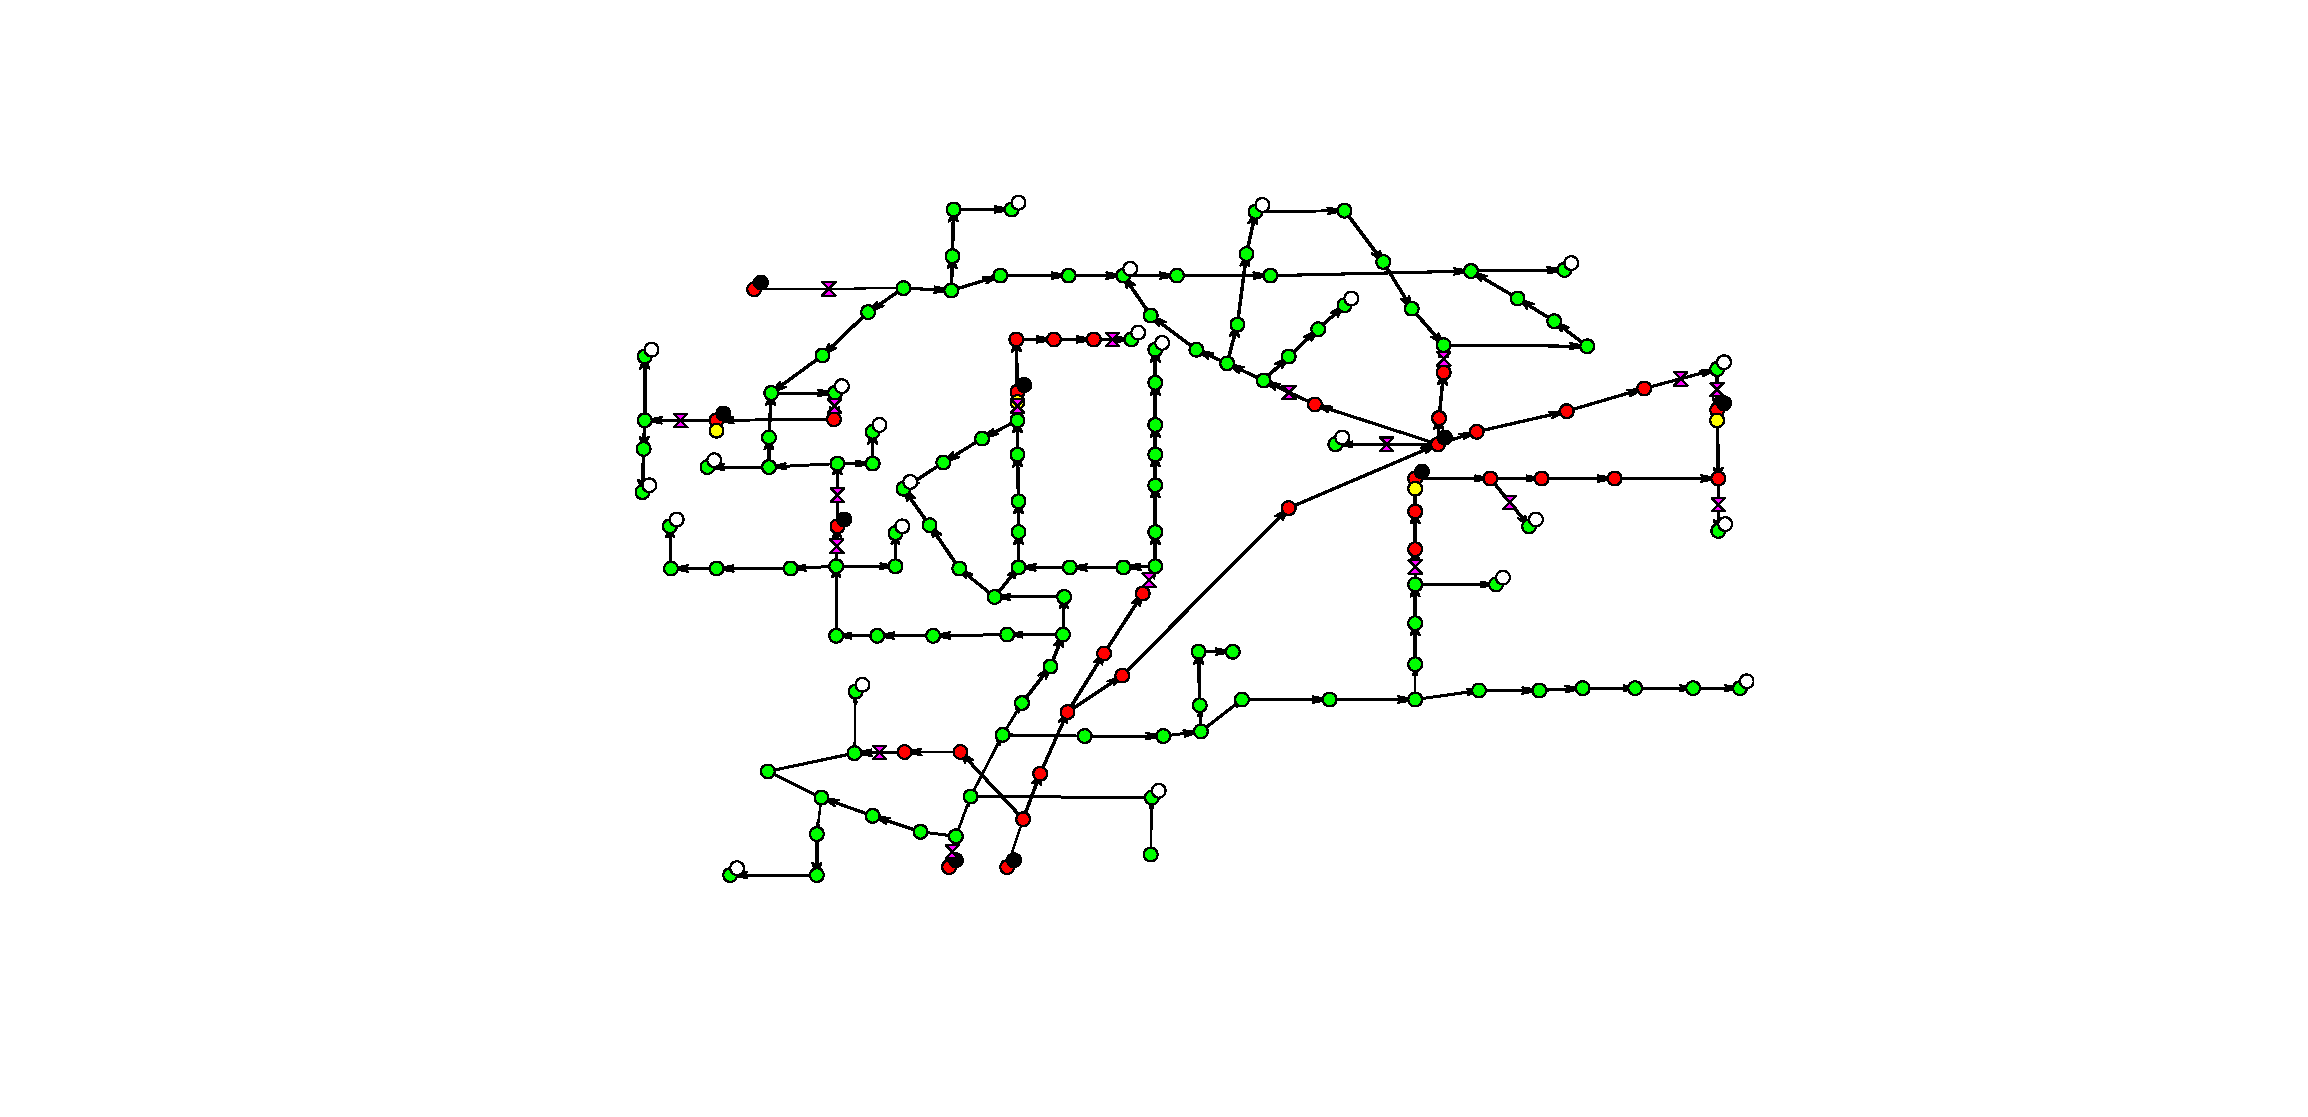
\includegraphics[width=\linewidth]{images/containment_attackAtOnce_9V}\caption{Scenario where all possible vulnerable nodes are always attacked simultaneously\protect \\
Green -- Demand partition\protect \\
Red -- Vulnerable partition\protect \\
Black -- Vulnerable nodes\protect \\
White -- Demand nodes}
\end{figure}



\subsection{\label{sub:Scenario-3:independent-vulnerable}Scenario of independent attacks}
\subsubsection{Key assumptions}
\begin{itemize}
    \item  Vulnerable nodes may be attacked independently, at different time points or not at all.
\end{itemize}


\subsubsection{Solution formulation}

Formulating as mixed integer linear optimization problem:

\begin{eqnarray*}
min & (\sum x_{i}+\sum z_{i})\\
sub\\
\mathbf{A}\left[\begin{array}{c}
\mathbf{x}\\
\mathbf{y}\\
\mathbf{z}\\
\mathbf{d}\\
\mathbf{w}\\
\mathbf{v}
\end{array}\right] & \leq & \mathbf{b}\\
\mathbf{A_{eq}}\left[\begin{array}{c}
\mathbf{x}\\
\mathbf{y}\\
\mathbf{z}\\
\mathbf{d}\\
\mathbf{w}\\
\mathbf{v}
\end{array}\right] & = & \mathbf{b_{eq}}
\end{eqnarray*}


Where $\mathbf{x}\equiv[x_{i}]$ is a decision variable vector whose
components are 1 if there exists a sensor at $i^{th}$node, 0 otherwise.

$\mathbf{y}\equiv[y_{i}]$ is a decision variable vector whose components
are 1 if $i^{th}$node is in the demands side of the actuators(demand
partition), 0 otherwise (source partition).

$\mathbf{z}\equiv[z_{i}]$ is a decision variable vector whose components
are 1 if there exists an actuator at $i^{th}$edge, 0 otherwise.

$\mathbf{d}\equiv[d_{i}]$ is a decision variable vector whose components
store $M-$the ``distance to detection'' for a particular vulnerable
node.

$\mathbf{w}\equiv[w_{i}]$ is 1 if $i^{th}$node is in the demand
partition, a large number ($M$) otherwise.

$\mathbf{v}\equiv[v_{ji}]$ is 1 if the $j^{th}$ vulnerable node's
distance to detection is inequal to the distance to the $i^{th}$
(sensor\ref{v-inequality-at-sensor-nodes}) node.

$M$ is a large number greater in order than the distances in the
network.

Hence the decision vector $\left[\mathbf{\begin{array}{cccccc}
\mathbf{x} & y & z & a & w & \mathbf{v}\end{array}}\right]$ is of length $3*N+E+V+N*V$, where $V$ is the number of vulnerable
nodes, $N$ is the number of nodes, $E$ is the number of edges.

$A=\left[\begin{array}{ccc}
A_{1} & \mathbf{0} & \mathbf{0}\\
\mathbf{0} & A_{2} & \mathbf{0}\\
\mathbf{} & A_{3}
\end{array}\right]$, $A_{eq}=\left[\begin{array}{ccc}
A_{eq1} & \mathbf{0} & \mathbf{0}\\
\mathbf{0} & A_{eq2} & \mathbf{0}\\
 & A_{eq3}
\end{array}\right]$, $b=\left[\begin{array}{c}
b_{1}\\
b_{2}\\
b_{3}
\end{array}\right]$, $b_{eq}=\left[\begin{array}{c}
b_{eq1}\\
b_{eq2}\\
b_{eq3}
\end{array}\right]$.

$A_{1}$ is a matrix of vulnerable nodes vs. affected nodes, with
$A_{1ij}=-1$ if $i^{th}$ vulnerable node affects the $j^{th}$ node
in graph.

$b_{1}=\left[\begin{array}{c}
.\\
.\\
.\\
-1\\
.\\
.\\
.
\end{array}\right]$

$A_{eq1}=b_{eq1}=\mathbf{\left[O\right]}$

To link the partitioning variables $\mathbf{y}$ to the variables
in the cost function, $\mathbf{z}$:

$A_{2}=\left[\begin{array}{cc}
J & I_{E\times E}\end{array}\right]$ where $J$ is the incidence matrix.

$b_{2}=\left[\mathbf{O}\right]$. The presence of an edge from source
to demand forces the corresponding $\mathbf{z}_{i}$ to switch to
one, indicating the presence of an actuator on that edge.

$A_{eq2}$, $b_{eq2}$ provide bounds to force the decision variables
to reality, viz. the demand nodes necessarily being in the demand
partition and the vulnerable nodes being in the source. We might also
include constraints to consider a few steps after vulnerable node
to be necessarily in the source partition, as done in \cite{palleti_actuator_2018}.

We use the shortest distances from each of the vulnerable nodes to
all other nodes in the graph to model time to contamination. We're
assuming the actual times are linear functions of distance. Let this
matrix be $\mathbf{D}$. The first set of constraints of $A_{3}$
is one for each entry in $\begin{array}{c}
M-\mathbf{D}\end{array}$ matrix, each of which is multiplied with $\mathbf{x}$. Each constraint
is balanced by $-d_{j}$, where $j$ is the vulnerable node under
consideration in that constraint. $b_{3}=\left[\mathbf{O}\right].$

Now, $d_{j}$ is greater than or equal to $M-D$$_{ij}$. We add constraints
to force equality to the distance to the closest sensor: $D_{ij}+d_{j}-Mv_{ij}\leq M$
for all sensors. \label{v-inequality-at-sensor-nodes}More constraints
for making sure non-sensor nodes don't use positive $v_{ij}$: $-x_{i}+v_{i}\leq0$.
For ensuring at least one equality of $D{}_{ij}$ and $d_{j}$, per
$j$: $A_{1j}\mathbf{x}-A_{j}\mathbf{v}_{j}\leq-1$.

The actuators need to be at least $M-d_{j}$ distance away from the
each of the vulnerable nodes. This can be implemented in two ways:
constraining the actuators to be placed after a particular distance,
or constraining the demand partition to start after a particular distance.
Since generally speaking $N<E$ in a lot of networks, we show the
node implementation.

Transform the $\mathbf{y}$ vector to $\mathbf{w},$ where $w_{i}=M$
denotes the sensor partition and $w_{i}=1$ implies the node is in
demand partition. Construct constraints for actuator placement for
the $i^{th}$node as follows: $\left[\begin{array}{ccccc}
... & 0 & -(M+D_{ij}-1) & 0 & ...\end{array}\right]\left[\mathbf{\mathbf{w}}\right]+\left[\begin{array}{c}
-1\end{array}\right]d_{j}\leq\left[\begin{array}{c}
-2*M\end{array}\right]$. This ensures that when $\mathbf{w}_{i}$ is $1$, the constraint
is activated and only satisfied if the corresponding $\mathbf{D_{ij}>d_{j}}$.
When $\mathbf{w}_{i}$ is $M$, the constraint is always satisfied
as $M^{2}$is several orders of magnitude greater than $2*M$.


\subsubsection{Small network example}

Consider the same network in Figure 1, with the two vulnerable nodes
(1, 2) and one demand node (6).

The additional constraints over case 2 introduced in this case are:
\begin{eqnarray*}
\left[\begin{array}{cccccc}
M-0 & 0 & 0 & 0 & 0 & 0\\
0 & M-1 & 0 & 0 & 0 & 0\\
0 & 0 & M-1 & 0 & 0 & 0\\
0 & 0 & 0 & M-2 & 0 & 0\\
0 & 0 & 0 & 0 & M-2 & 0\\
0 & 0 & 0 & 0 & 0 & M-3
\end{array}\right]\mathbf{x}-\left[\begin{array}{c}
d_{1}\\
d_{1}\\
d_{1}\\
d_{1}\\
d_{1}\\
d_{1}
\end{array}\right] & \leq & \left[\begin{array}{c}
0\\
0\\
0\\
0\\
0\\
0
\end{array}\right]\\
\left[\begin{array}{cccccc}
M-M & 0 & 0 & 0 & 0 & 0\\
0 & M-0 & 0 & 0 & 0 & 0\\
0 & 0 & M-1 & 0 & 0 & 0\\
0 & 0 & 0 & M-1 & 0 & 0\\
0 & 0 & 0 & 0 & M-1 & 0\\
0 & 0 & 0 & 0 & 0 & M-2
\end{array}\right]\mathbf{x}-\left[\begin{array}{c}
d_{2}\\
d_{2}\\
d_{2}\\
d_{2}\\
d_{2}\\
d_{2}
\end{array}\right] & \leq & \left[\begin{array}{c}
0\\
0\\
0\\
0\\
0\\
0
\end{array}\right]\\
\end{eqnarray*}
This gets us variables storing $M-d_{i}$, the value after subtracting
the minimum distance to sensor from the large number for each vulnerable
node.

Constraints for ensuring the conditions around $d_{j}$'s:

\begin{eqnarray*}
\left[\begin{array}{cccccc}
0 & 0 & 0 & 0 & 0 & 0\\
0 & 1 & 0 & 0 & 0 & 0\\
0 & 0 & 1 & 0 & 0 & 0\\
0 & 0 & 0 & 2 & 0 & 0\\
0 & 0 & 0 & 0 & 2 & 0\\
0 & 0 & 0 & 0 & 0 & 3
\end{array}\right]\mathbf{x}+\left[\begin{array}{c}
d_{1}\\
d_{1}\\
d_{1}\\
d_{1}\\
d_{1}\\
d_{1}
\end{array}\right]-M\left[\begin{array}{c}
v_{11}\\
v_{12}\\
v_{13}\\
v_{14}\\
v_{15}\\
v_{16}
\end{array}\right] & \leq & M\left[\begin{array}{c}
1\\
1\\
1\\
1\\
1\\
1
\end{array}\right]\\
\left[\begin{array}{cccccc}
M & 0 & 0 & 0 & 0 & 0\\
0 & 0 & 0 & 0 & 0 & 0\\
0 & 0 & 1 & 0 & 0 & 0\\
0 & 0 & 0 & 1 & 0 & 0\\
0 & 0 & 0 & 0 & 1 & 0\\
0 & 0 & 0 & 0 & 0 & 2
\end{array}\right]\mathbf{x}+\left[\begin{array}{c}
d_{2}\\
d_{2}\\
d_{2}\\
d_{2}\\
d_{2}\\
d_{2}
\end{array}\right]-M\left[\begin{array}{c}
v_{21}\\
v_{22}\\
v_{23}\\
v_{24}\\
v_{25}\\
v_{26}
\end{array}\right] & \leq & M\left[\begin{array}{c}
1\\
1\\
1\\
1\\
1\\
1
\end{array}\right]\\
\end{eqnarray*}


For $v_{i}$'s are 1 only when $i$ is a sensor:$-x_{i}+v_{i}\leq0$.
At least one equality constraint being satisfied:

\begin{eqnarray*}
\left[\begin{array}{cccccc}
-1 & -1 & -1 & -1 & -1 & -1\\
0 & -1 & -1 & -1 & -1 & -1
\end{array}\right]\mathbf{x}-\left[\begin{array}{cccccc}
1 & 1 & 1 & 1 & 1 & 1\\
0 & 1 & 1 & 1 & 1 & 1
\end{array}\right]\left[\begin{array}{c}
\mathbf{v_{1}}\\
\mathbf{v_{2}}
\end{array}\right] & \leq & \left[\begin{array}{c}
-1\\
-1
\end{array}\right]\\
\end{eqnarray*}


The constraints for ensuring desired partitioning are:

\begin{eqnarray*}
-1\times\left[\begin{array}{cccccc}
M+0-1 & 0 & 0 & 0 & 0 & 0\\
0 & M+1-1 & 0 & 0 & 0 & 0\\
0 & 0 & M+1-1 & 0 & 0 & 0\\
0 & 0 & 0 & M+2-1 & 0 & 0\\
0 & 0 & 0 & 0 & M+2-1 & 0\\
0 & 0 & 0 & 0 & 0 & M+3-1
\end{array}\right]\mathbf{w}-\left[\begin{array}{c}
d_{1}\\
d_{1}\\
d_{1}\\
d_{1}\\
d_{1}\\
d_{1}
\end{array}\right] & \leq & \\ \left[\begin{array}{c}
\begin{array}{c}
-2M\\
-2M\\
-2M\\
-2M\\
-2M\\
-2M
\end{array}\end{array}\right]
&&\\
-1\times\left[\begin{array}{cccccc}
M+M-1 & 0 & 0 & 0 & 0 & 0\\
0 & M+0-1 & 0 & 0 & 0 & 0\\
0 & 0 & M+1-1 & 0 & 0 & 0\\
0 & 0 & 0 & M+1-1 & 0 & 0\\
0 & 0 & 0 & 0 & M+1-1 & 0\\
0 & 0 & 0 & 0 & 0 & M+2-1
\end{array}\right]\mathbf{w}-\left[\begin{array}{c}
d_{2}\\
d_{2}\\
d_{2}\\
d_{2}\\
d_{2}\\
d_{2}
\end{array}\right] &\leq &\\  \left[\begin{array}{c}
\begin{array}{c}
-2M\\
-2M\\
-2M\\
-2M\\
-2M\\
-2M
\end{array}\end{array}\right]&&
\end{eqnarray*}



\subsubsection{Results and verification}

The network is verified to have no paths from vulnerable to demand
after removing edges. The distance to detection is always lesser than
the distance to the first actuators.

\begin{table}[ht]
\begin{tabular}{|c|c|c|c|}
\hline
Vulnerable Nodes & Time to sense & Sensor nodes & Actuator edges\tabularnewline
\hline
\hline
    1 2 3 19 32 37 39 53 66 & 0 0 0 0 0 0 0 0 0 &\begin{tabular}[c]{@{}c@{}} 1 2 3 19 32\\37 39 53 66 \end{tabular} &\begin{tabular}[c]{@{}c@{}} 1 4 40 48 51 52 68 \\150 151 152 153 149\end{tabular}\tabularnewline
\hline
1 2 3 & 0 0 0 & 1,2,3 & 1,4,68\tabularnewline
\hline
    1 2 3 19 32 37 39 53 66\footnote{all nodes 1 distance downstream are considered source partition} & 0 4 1 0 1 0 0 1 0 &\begin{tabular}[c]{@{}c@{}}  1 7 19 33 \\37 39 54 57 66 \end{tabular} &\begin{tabular}[c]{@{}c@{}} 2 8 12 30 38 40 48 \\51 52 67 69 77 78 89 103 108 110\end{tabular}\tabularnewline
\hline
\end{tabular}\caption{The distance to detection for different sets of vulnerable nodes}
\end{table}


In the previous work \cite{palleti_actuator_2018}, the similar task was partial shutdown
of WDN. The number of actuators suggested was 20 viz. 2, 12, 16, 24,
30, 38, 40, 48, 51, 52, 67, 71, 76, 86, 79, 89, 108, 110, 127, 112
with 3 sensors (at nodes 40, 54, 67) and the same 9 vulnerable nodes.
The nodes directly downstream of vulnerable are taken as source nodes.
Here for task 4, we get a solution with 26 cardinality: 17 actuators,
9 sensors. The previous work does not require that no demand node
be compromised though.

\begin{figure}[ht]
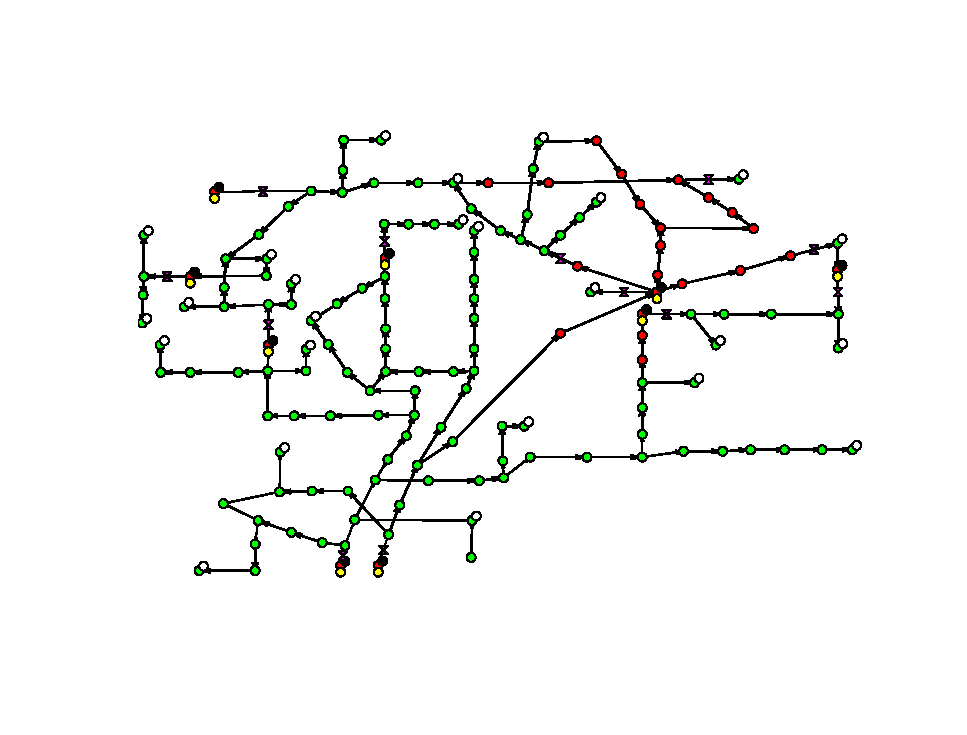
\includegraphics[width=\linewidth]{images/zoneContainment_9sources}\caption{Sensor and actuator placement strategy for 9 vulnerable nodes\protect \\
Green -- Demand partition\protect \\
Red -- Vulnerable partition\protect \\
Black -- Vulnerable nodes\protect \\
White -- Demand nodes\protect \\
Yellow -- sensor nodes}
    \label{fig:zoneContainment_9sources}
\end{figure}
\begin{figure}[ht]
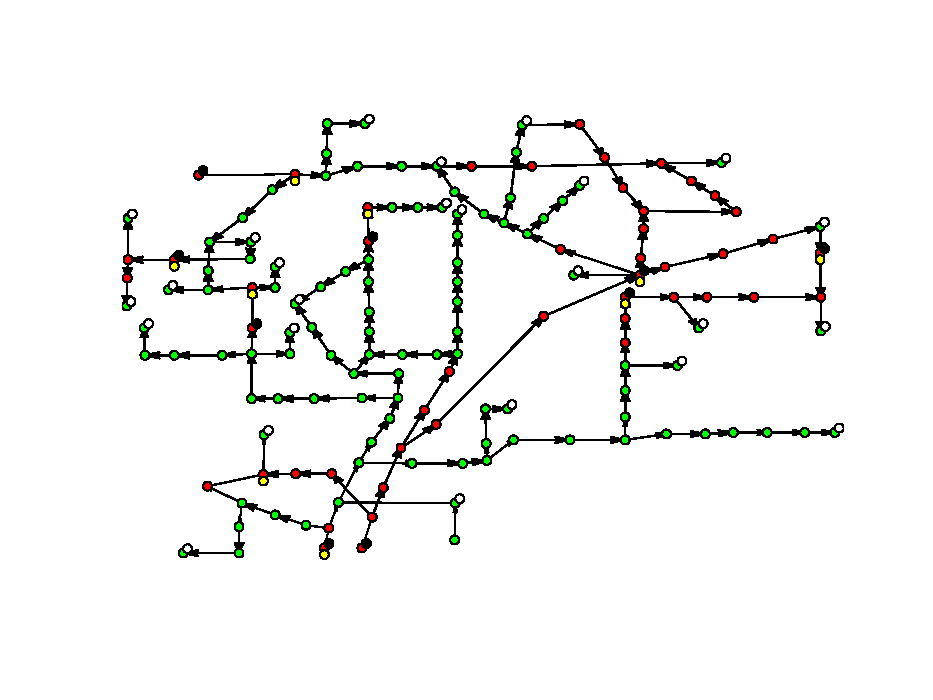
\includegraphics[width=\linewidth]{images/containment_9sources_1downstreamSourceEach}\caption{Sensor and actuator placement strategy for 9 vulnerable nodes and
instant downstream contamination\protect \\
Green -- Demand partition\protect \\
Red -- Vulnerable partition\protect \\
Black -- Vulnerable nodes\protect \\
White -- Demand nodes\protect \\
Yellow -- sensor nodes}
    \label{fig:containment_9sources_1downstreamSourceEach}
\end{figure}



\section{Validation of \cite{palleti_actuator_2018}}
The results of the scenario explored in \cite{palleti_actuator_2018} are presented in \autoref{fig:cardinality21-Venkat-results-reproduced}
\begin{figure}[!hptb]
\protect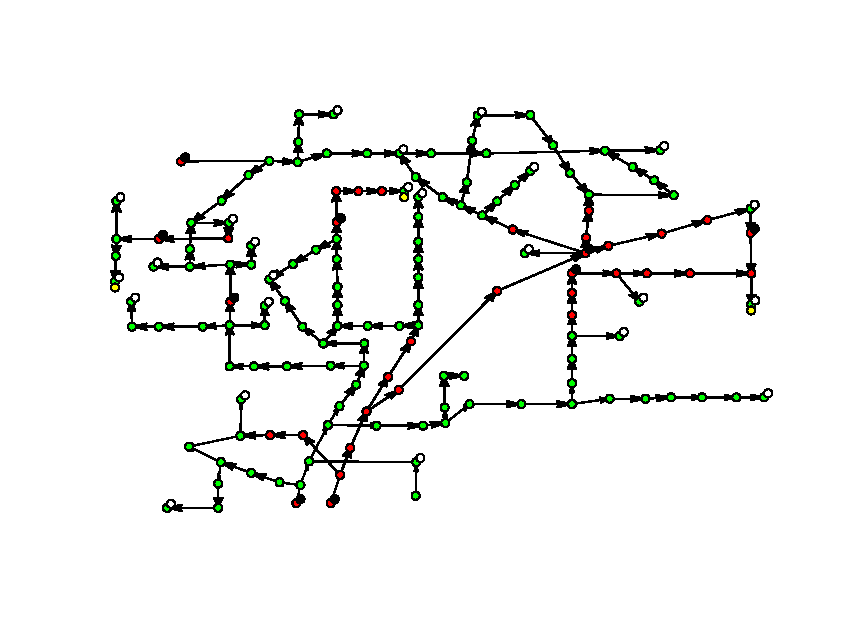
\includegraphics[width=\linewidth]{images/cardinality21_Venkat_results_reproduced}\protect\caption{Validation of \cite{palleti_actuator_2018}, case of allowing demand nodes to be compromised
\protect \\
The cardinality is 21, the same as presented in the earlier work.}

    \label{fig:cardinality21-Venkat-results-reproduced}
\end{figure}



\section{Conclusions and future work}

For a given WDN, we presented ways to arrive at a sensor and actuator
placement strategy. This sensor and actuator network design is useful
for water authorities to detect contaminants and isolate the contaminated
area in the event of an attack on the WDN. We proposed a multi-objective
linear programming formulation that gives the optimal sensor and actuator
cardinality.

The formulation can reproduce the results of \cite{palleti_actuator_2018} after relaxing
the full requirements to partial, viz. to prevent further contamination
of demand nodes.

A performance benchmark of the simultaneous framework and the sequential
non-linear optimization solution would be an illuminating exercise.

This formulation introduces an $O(NV)$ blowup in the number of decision
variables, but there exist techniques to solve such specifically constrained
variables much faster. An implementation using such techniques would
be useful for assessing real performance.

Integration of an implementation of these algorithms with existing
open-source toolboxes for sensor and actuator placement is a possible
future action, which makes the techniques presented here much more
accessible.

\section{REFERENCES}
%\begin{thebibliography}{00}
\bibliographystyle{elsarticle-harv}
\bibliography{jpaper}

\batchmode
\end{document}
